%-*- coding: UTF-8 -*-
% gougu.tex
% 勾股定理
\documentclass[UTF8,c5size]{ctexart} 
% ctexart, ctexrep, ctexbook 分别用来写中文短文,中文报告,中文书籍 
% ctexart默认时标题不独自成页的,可加入选项titlepage修改为独自成页
% c5size表示正文正五号字体
% 2.4.1
\usepackage{graphicx}
% 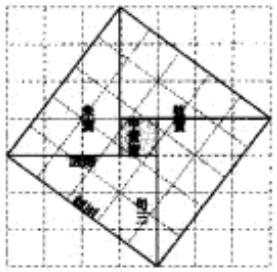
\includegraphics[scale=0.6]{xiantu.png}
\usepackage{float}
% \begin{table}[H] 
\usepackage{amsmath}
% 满足式\eqref{eq:gougu}的整数称为\emph{勾股数}。
\usepackage{geometry}
\geometry{a4paper,centering,scale=0.8}
% 设计页面尺寸
\usepackage[format=hang,font=small,textfont=it]{caption}
% 改变图标标题格式
\usepackage[nottoc]{tocbibind} 
% tocbibind默认把章节目录、图标目录、文献、索引加入章节目录里
% 选项可进行进一步控制,nottoc不加入章节目录(默认目录自己会出现在目录里)
% 3.1.2
\newenvironment{myquote}
{\begin{quote}\kaishu\zihao{-5}}
{\end{quote}}
% 定义新环境
\newcommand\degree{^\circ} 
% 定义新命令
% ^表示上标,\circ表示函数复合的二元运算符。
% _表示下标
% 数学符号4.3

\newtheorem{thm}{定理}
% 定理类环境
% 2.2.4


\title{\heiti 杂谈勾股定理}
\author{\kaishu 张三}
\date{\today}
% title author date 可以放在maketitle前的任何位置,通常放在导言区 date可以省略,默认为今天

\bibliographystyle{plain}
% \bibliographystyle命令设定参考文献格式,通常在导言区完成。
% 基本的Bibtex文献格式包括plain、unsrt、alpha和abbrv
% plain格式按作者、日期标题排序
% 文档中使用\cite引用文献
% 文档中用\nocite命令指明不引用但仍列出文献标签
% \bibliography{math}指明文献库
% 引用bib文献,需
% a、先xelatex *.tex源文件编译,将\cite,\bibliography,\bibliographystyle写入.aux辅助文件,生成无文献PDF
% b、然后运行bibtex *.aux生成.bbl文献列表
% c、xelatex *.tex,依靠*.aux *.bbl生成有文献无引用PDF,同时将\cite应用信息写入.aux
% d、xelatex *.tex,依靠*.aux *.bbl,在应用处生存引用信息,得到最终PDF
% 可使用JabRef生存.bib
% 3.3.1

%这里之前称为导言区preamble,这里正式开始文档
\begin{document}

\maketitle
% \maketitle通常为document的第一个指令,前面的ctexart默认不单独成页,ctexrep、ctexbook默认单独成页
% 可通过文档类选项notitlepage修改不单独成页
% title可不通过\title \maketitle命令得到,直接手工排版得到,
% 2.3.1

\begin{abstract}
        这是一篇关于勾股定理的小短文。
\end{abstract}

\tableofcontents
% 读入.toc目录文件如果存在的话
% ctexart为section subsection subsubsection 三级目录
% ctexrep、ctexbook为chapter section subsection 三级目录
% 可以通过修改计数器tocdepth来控制目录的深度 
% 3.1.1
% 3.1.2

\section{勾股定理在古代}
% ctexart的最高层
% ctexrep、ctexbook的最igaocheng为chapter
% 三种文档类还有一个可选的最高层part
% \appendix为附录开始,改用字母标号
% 2.3.2 表2.13 章节层次
        西方称勾股定理为毕达哥拉斯定理,
        将勾股定理的发现归功于公元前 6 世纪的毕达哥拉斯学派\cite{Kline}。
        该学派得到了一个法则,可以求出可排成直角三角形三边的三元数组。
        毕达哥拉斯学派没有书面著作,该定理的严格表述和证明则见于
        欧几里德\footnote{欧几里德,约公元前 330--275 年。}
        《几何原本》的命题 47:
        “直角三角形斜边上的正方形等于两直角边上的两个正方形之和。”
        证明是用面积做的。

        我国《周髀算经》载商高(约公元前 12 世纪)答周公问:
        \begin{myquote}
                勾广三,股修四,径隅五。
        \end{myquote}
        又载陈子(约公元前 7--6 世纪)答荣方问:
        % --将输出一个"en dash",即宽度与字符n相当的短线
        \begin{myquote}
                若求邪至日者,以日下为勾,日高为股,勾股各自乘,
                并而开方除之,得邪至日。
        \end{myquote}
        都较古希腊更早。后者已经明确道出勾股定理的一般形式。
        图\ref{fig:xiantu}是我国古代对勾股地定理的一种证明\cite{quanjing}。
	\begin{figure}[ht]
	        \centering
	        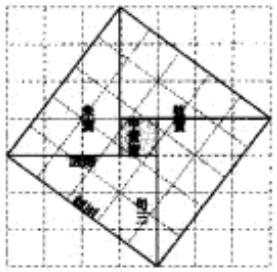
\includegraphics[scale=0.6]{xiantu.png}
            % graphicx宏包
	        \caption{宋赵爽在《周髀算经》注中作的弦图(仿制),
	                该图给出了勾股定理的一个极具对称美的证明。}
	        \label{fig:xiantu}
	\end{figure}
    % figure环境可选参数[ht],表示浮动可以出现在环境周围的文本所在处here和一页的top。
    % figure环境内部相当与普通的段落(默认没有缩进);
    % \centering 表示后面的内容居中;
    % \includegraphics插入图片
    % \caption加自动编号和标题
    % \lable加上标签,其他地方可用\ref{fig:xiantu}引用


\section{勾股定理在近代形式}
        勾股定理可以用现代语言表述如下:
        \begin{thm}[勾股定理]
                直角三角形斜边的平方等于两腰的平方和。

                可以用符号语言表述为:设直角三角形ABC,
                其中$\angle C = 90\degree$,则有
                % 用$a+b$可以得到漂亮的数学公式a+b
                \begin{equation}\label{eq:gougu}
                        AB^2 = BC^2 + AC^2.
                \end{equation}
                % 比较重要的公式使用equation黄金可以方便的进行引用
        \end{thm}
        满足式\eqref{eq:gougu}的整数称为\emph{勾股数}。
        第1节所说的毕达哥拉斯学派得到的三元数组就是勾股数。
        下表列出了一些较小的勾股数:
        \begin{table}[H]
                \begin{tabular}{|rrr|}
                \hline
                直角边 $a$ & 直角边 $b$ & 斜边 $c$ \\
                \hline
                3 &      4 &     5\\
                5 &     12 &    13\\
                \hline
                \end{tabular}%
                \qquad ($a^2 + b^2 = c^2$)
        \end{table}
        % tabular参数|rrr|声明了又三列右对齐
        % 行之间用\\隔开
        % 每行表项用&隔开
        % 横线哦你个\hline产生
        % 并排隔开用\qquad,产生一个2em(大约两个‘M’宽度)的空白
        % \end{tabular}后的%可取消掉换行产生的多余空格(为毛)
        % 表格与figure格式差不多,这表格没有用\caption产生标题
        % 由于前面下表列出了...,文体构造上不允许表格移动,
        % table后面的选项H表示表格放这里不移动,
        % H由float宏包提供

\nocite{Shiye}
% 没引用但仍在参考文献李输出
\bibliography{math}
% 跟前面的\bibliographystyle{plain}对应,指明使用math.bib数据库,多个文献用逗号隔开
\end{document}


